\chapter{Unsupervised learning}
\label{cha:unsupervised}

While for supervised models we use labelled examples, for unsupervised we do not have any labels, but only data.

\section{Clustering}

\subsection{K-means clustering}
        This is a quite popular naive approach for clustering. This method assumes that you decide a priori the number of clusters. Each cluster will be represented by its mean $\mu_i$. The idea is to assign example to the clusters with the closer mean.\\

        The algorithm works within this line:
        \begin{enumerate}
            \item initialize cluster means $\mu_1, \dots, \mu_n$ (a way of doing it is at random)
            \item iterate until no mean changes:
            \begin{enumerate}
                \item assign each example to cluster with nearest mean
                \item update cluster means according to assigned examples
            \end{enumerate}
        \end{enumerate}

        This is a very simple approach, it is still used especially when we have some form of processing (dimensionality reduction ...) that maps example in low dimensional space, where k-means is sufficient. \\
        Combined with other approached is still something that is currently used frequently.
        

    \subsection{Distance metrics}
        In order to compute some clustering, we need to define a metric for the concept of "distance" (aka notion of \textit{similarity}), here we report the main metrics that can be used:
        \begin{enumerate}
            \item \textbf{standard euclidean distance in $\R^d$}: is the most natural choice, it is a instance of a more general metric (Minkowski, see next point)
            $$d(\pmb{x}, \pmb{x}') = \sqrt{\sum _{i=1} ^ d (\pmb{x}_i - \pmb{x}_i ')^2}$$
            \item \textbf{generic Minkowski metric for $p \geq 1$}:
            $$d(\pmb{x}, \pmb{x}') = \left(\sum _{i=1} ^ d |\pmb{x}_i - \pmb{x}_i '|^p \right)^{1/p}$$ If we replace $p=2$ we get the euclidean distance while if $p=1$ we get the Manhattan distance.
            \item \textbf{Cosine similarity (cosine  of the angle between two vectors)}: this is just the dot product divided by the two norms.
            $$s(\pmb{x}, \pmb{x}') = \frac{\pmb{x}^T \pmb{x}'}{||\pmb{x}|| ||\pmb{x}'||}$$
      \end{enumerate}

      It is also possible to use metric learning: instead of assuming a pre-defined metric, we can learn metric from data.

    \subsection{Quality of clustering}
        There are a number of criteria for defining a quality of clusters, here we present just one, quite intuitive: \textbf{Sum-of-squared error criterion}. 
        This method tells me how bad the approximation of the cluster is using the means.\\

        For each cluster, we take the mean $\mu_i$ (as general measure, not only k-means) within each cluster. I compare all examples ($n_i$ number of samples) in the cluster with the mean of the cluster they are in. The error will be computed as the squared error (sample and mean): 
        $$\mu_i = \frac{1}{n_i} \sum_{\pmb{X} \in \mathcal{D}_i} \pmb{x}$$
        The sum-of-squared errors is defined as the sum over the totality of clusters
        $$E = \sum _{i=1}^k \sum_{\pmb{X} \in \mathcal{D}_i} || \pmb{x} - \mu_i|| ^ 2$$
        This basically tells us how bad the approximation of a cluster is using the means. 

\section{Gaussian Mixture Model (GMM)}
        The idea is again assuming a priori the number of clusters I want to get, then I suppose that each cluster is represented as a Gaussian distribution. I need to estimate the mean and possibly the variance (or co-variance) of the Gaussian distribution.

        \begin{figure}[ht]
            \centering
            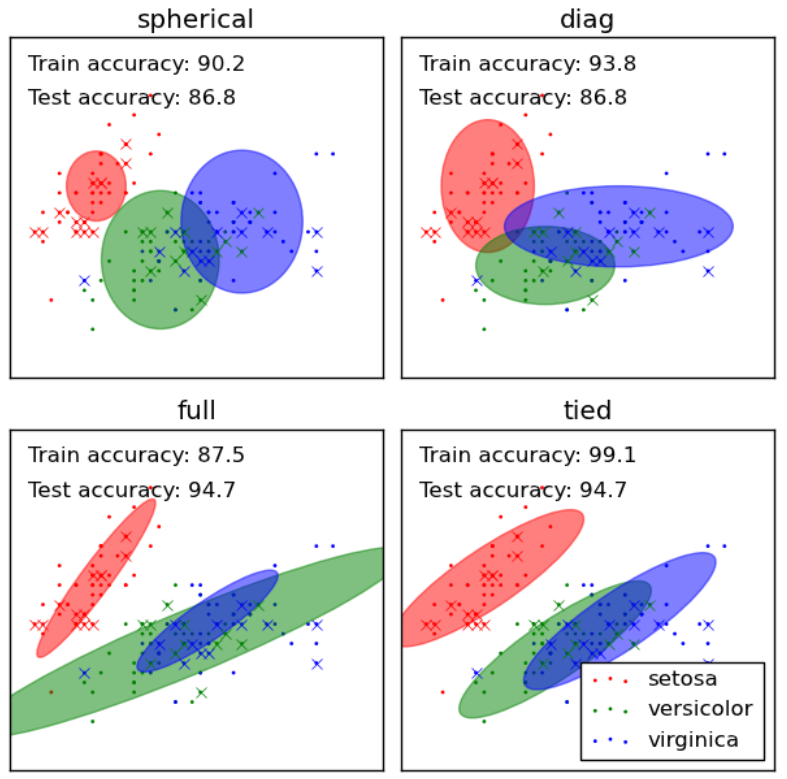
\includegraphics[scale=0.5]{images/GMM.png}
            \caption{GMM clustering for the same data with different parameters}
            \label{fig:GMM}
        \end{figure}

        In this Figure \ref{fig:GMM}, we represent ways in which we can use variances in different dimensions:
        \begin{enumerate}
            \item \textbf{Spherical}: we use same variance for each dimension and for each cluster
            \item \textbf{Diagonal}: we use diagonal variance (axis aligned gaussians), we can still have different spreads in different dimensions
            \item \textbf{Tied}: in this case we also introduce covariance (estimate relationships between features), shared (tied) between different clusters. 
            \item \textbf{Full}: in this example we see a full solution, in which we can have different co-variances matrices for different clusters.
        \end{enumerate}
        This is an example of different ways of fitting the same data, so based on the approach we select we can get different solutions.\\

        \subsection{Spherical GMM}
            This is the easier way of using GMM, therefore mean estimation. Of course the problem of applying GMM, we need to estimate parameter, but we can no longer use maximum likelihood estimation because we do not have any label for the data. 
            Here is an example of the so called \textit{Latent Variables} (which consists in a probability of assigning the sample to each cluster). Based on this, we can do Expectation Maximization.
            \begin{enumerate}
                \item start with initialization of parameters, 
                \item we compute the expected value for the latent variables (expected value for clusters assignment)
                \item using this expected value, we maximize the likelihood through the parameters
                \item this gives me a new value of the parameter and then iterate until convergence
            \end{enumerate}
            

            \textbf{Settings}:
            \begin{itemize}
                \item A dataset of $n$ examples
                \item for each example $x_i$, a cluster assignment (the latent variable) is modelled as $z_{i1}, \dots, z_{ik}$ (for each sample, a value for each cluster) modelled with a one-hot encoding (vector of binary variables, we have 1 only for the correct class, 0 otherwise)
                \item we assume for simplicity that we are only estimating the mean of the gaussian, the variance is assumed to be known
            \end{itemize}
            

            \textbf{General Algorithm}:
            \begin{enumerate}
                \item initialize $h = {\mu_1, \dots, \mu_k}$ as hypothesis, initialization randomly
                \item iterate until the difference in maximum likelihood is below a certain threshold:
                \begin{enumerate}
                    \item \textbf{E-step}: calculate the expected value $E[z_{ij}]$ of each latent variable assuming that the current hypotheses holds.
                    \item \textbf{M-step}: calculate new maximum likelihood values (new hypothesis) $h' = {\mu_1, \dots, \mu_k}$ assuming values of latent variables are their expected values. Replace $h$ with $h'$.
                \end{enumerate}
            \end{enumerate}
            

            \textbf{Compute the expected value $z_{ij}$}
            \begin{enumerate}
                \item \textbf{E-step}: computing the probability that example $x_i$ comes from Gaussian$_j$, assuming that we known the means and the variances of the Gaussian
                $$E[z_{ij}] = \frac{p(x_i|\mu_j)}{\sum _{l=1} ^ k p(x_i|\mu_l)} =   
                \frac   {e^{- \frac{1}{2 \sigma^ 2} (x_i -\mu_j)^2 }}
                        { \sum _{l=1} ^ k e^{- \frac{1}{2 \sigma^ 2} (x_i - \mu_l)^2 }}$$
                The coefficients of the Gaussian distributions is omitted because can be simplified (is the variance is shared).
                This is a soft assignment. 
                \item \textbf{M-step}: perform maximum likelihood of the means $\mu_j '$ assuming that the latent variables are given by the expectations. The result is:
                $$\mu_j ' = \frac{ \sum_{i=1}^ n E[z_{ij}] x_i} {\sum _{i=1} ^ n E[z_{ij}]}$$
                If we know which example comes from which Gaussian, therefore we can be satisfied with the sample mean, but we do not know the belongings of the sample to the class. Here we know an \textit{expectation} of belonging to classes (in terms of probability), therefore we do not have a zero-one value, but as continuous probability, which can be seen as an assignment to a class weighted to a certain probability.
            \end{enumerate}
            
            \textbf{Expectation maximization}:\\
            This is a general strategy used to deal with optimization and maximization of the parameters of the hypothesis, in a setting in which I have unobserved data. Generally I have a dataset made of observed part $X$ and unobserved part $Z$.
            We would like to estimate the hypothesis maximizing the (log) likelihood of the data, where the latter include both $X, Z$. 
            $$h^* = \text{argmax}_h E_Z [ln \quad p(X, Z | h)]$$
            We want to maximize given the expectation of $Z$. Unobserved data $Z$ should be treated as random variables governed by the distribution depending on both $X, h$. The fact is that we do not know $h$, which is indeed the variable we want to estimate.\\
            The iterative procedure is described as follows:
            \begin{enumerate}
                \item initialize hypothesis $h$
                \item iterate until convergence
                \begin{enumerate}
                    \item \textbf{E-step}: compute the expected (log) likelihood of an hypothesis $h'$ for the full data, where the unobserved data distribution is modelled according to the current hypothesis $h$ (from previous iterations) and the observed data as
                    $$Q(h', h) = E_Z[ln (p(X, Z | h'))|h, X]$$
                    The expectation for the missing data $Z$ (in GMM is the cluster assigment vector) is computed with respect to $h, Z$ which are given by the last iteration and the known data.
                    \item \textbf{M-step}: replace the current hypothesis with the one maximizing $Q(h', h)$
                    $$h \leftarrow \text{argmax}_{h'} Q(h', h)$$
                \end{enumerate}
            \end{enumerate}

            This procedure is guaranteed to converge but it is likely to get to a local optimum. We can start with a good initialization coming from different methods. \\

            The results for a GMM are:
            $$p(x_i, z_{i1}, \dots, z_{ik} | h') = 
            \frac{1}{\sqrt{2 \pi} \sigma}       
            e^ {
            \left[ 
                - \sum _{j=1} ^k z_{ij} \frac{(x_i - \mu_j ') ^2}{2 \sigma ^2}
            \right]}
            $$

            In which any generic $x$ is $x_i$ and $z$ is a vector for each $x$ and each of the possible clusters (one-hot encoding). We can model the right end side with a Gaussian distribution, but instead of having a single mean, we get all differences $(x_i - \mu_j ') ^2$ and then we sum them up in some way that is weighted with the cluster assignment probability $z_{ij}$. 
            If $z_{ij}$ is one-hot, we will recover a single Gaussian, otherwise we will have a mixture. \\

            If I compute the log likelihood on the full dataset: 
            $$ln(p(X, Z| h)) = 
            \sum _{i=1} ^n 
            \left(
            ln \frac{1}{\sqrt{2 \pi} \sigma}
                - \sum _{j=1} ^k z_{ij}
                    \frac{(x_i - \mu_j ' )^2}{2 \sigma ^ 2}
            \right)
            $$
            This is just log of product over the example of the likelihood (properties of logarithm used on the previous formula). \\
            
            What we still need is the expectation over $E_Z[\dots]$. This is computed as follows: 
            \begin{align*}
                E_Z [ln ( p (Z, X| h'))] & = E_Z 
                                            \left[ \sum _{i=1} ^ n \left(
                                            ln \frac{1}{\sqrt{2 \pi} \sigma}
                                            - \sum _{j=1} ^k z_{ij}
                                                \frac{(x_i - \mu_j ' )^2}{2 \sigma ^ 2}
                                            \right) \right]\\
                                        & = \sum _{i = 1} ^ n 
                                        \left( 
                                        ln \frac{1}{\sqrt{2 \pi} \sigma}
                                        - \sum _{j=1} ^k E [z_{ij}]
                                                \frac{(x_i - \mu_j ' )^2}{2 \sigma ^ 2}
                                        \right)
            \end{align*}    
            While the expectation of the $x_i$ data comes from the $j$-th cluster, given current hypothesis $h$ and observed data $X$ is computed as:
            \begin{align*}
                E[z_{ij}]   &= \frac{p(x_i | \mu_j)}{\sum _{l=1} ^ k p(x_i | \mu_l)}\\
                            &= 
                            \frac   {e^{- \frac{1}{2 \sigma^ 2} (x_i -\mu_j)^2 }}
                                    { \sum _{l=1} ^ k e^{- \frac{1}{2 \sigma^ 2} (x_i - \mu_l)^2 }}
            \end{align*}
            The expectation of the log-likelihood is computed with $h'$ while the second is computed starting from $h$ (the old one, therefore this quantity is computable). Given that I have the formula of the likelihood, then I can maximize it.\\
            The next step is taking this expectation and then I perform maximization over the new hypothesis. \\
            The likelihood maximization gives this first result (since there is a minus sign, we can minimize instead of maximize), then we can set the derivation equal to zero with respect to $\mu_j '$ in order to find the maximum (in the example we are considering just one specific $\mu_j$ instead summing for every component).
            \begin{figure} [ht]
                \centering
                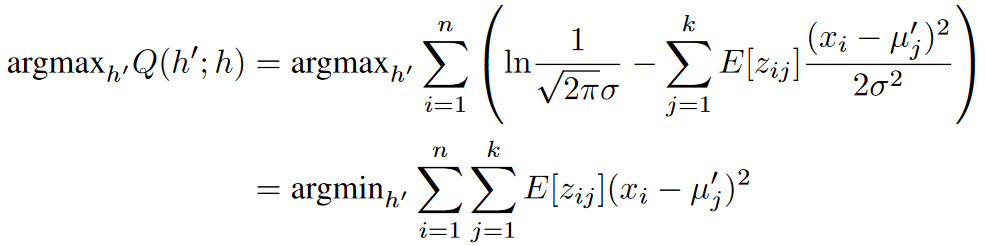
\includegraphics[scale=0.4]{images/m-step_GMM_maximization.png}
            \end{figure}
            \begin{figure} [ht]
                \centering
                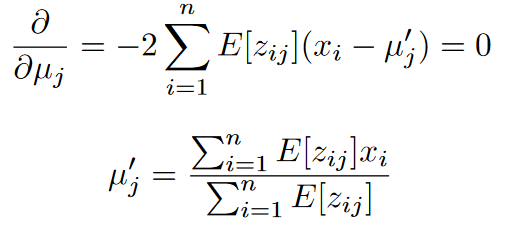
\includegraphics[scale=0.4]{images/m-step_GMM_zeroing.png}
            \end{figure}

        \subsection{How to choose the number of clusters}
            Up to now, we only assumed that we are given in advanced the number of clusters, but of course it is not always the case. 
            In some cases, having background helps us to understand the number of clusters should use, in general we can try to find out the number of cluster automatically by trying different values and look for the best one.
            There are some methods that can be used for this purpose: 
            \begin{itemize}
                \item \textbf{Elbow method}: based on the squared errors, if we increase the number of clusters, this quality measure drops (the edge case in which every example is by its own a cluster has an error equal to zero). 
                We need to find a solution for the trade-off between the number of  clusters and the means squared error: this method checks whether increasing the number of clusters is worth it or not. 
                We run the clustering (any kind) with an increasing number of clusters and we plot (Figure \ref{fig:elbow_method}) the error measure: in the curve we get we look for an "elbow", therefore a threshold for which we should stop increasing the number of clusters (drop in error starts to be less important).
                This method is a bit ambiguous, there is no formal procedure to do decide a point over another.
                \begin{figure}
                    \centering
                    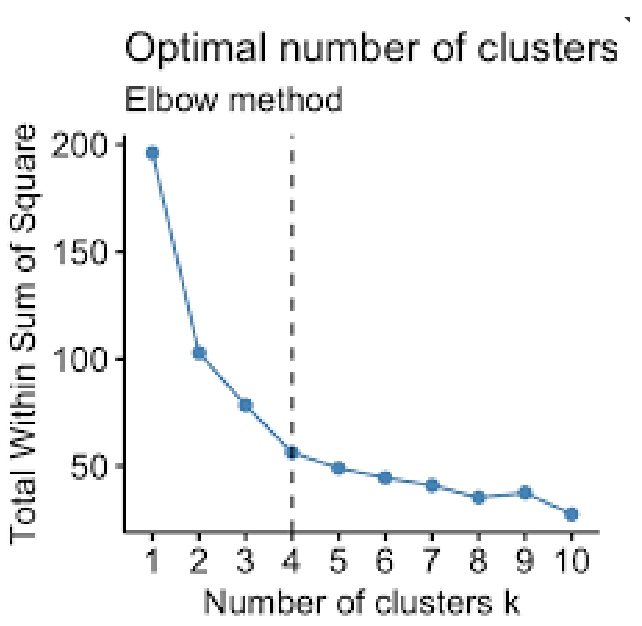
\includegraphics[scale=0.3]{images/elbow method.png}
                    \caption{Plot of the error rate within the increase of the number of clusters}
                    \label{fig:elbow_method}
                \end{figure}
                \item \textbf{Average silhouette}: this method gives us a precise definition for the number of clusters. This is based on the fact that by increasing the number of clusters, each of them becomes more homogeneous. But on the other hand also different clusters also become similar to each other (splitting data further). We need to look for inter-clusters dissimilarity (not only intra-clusters similarity).\\
                The procedure is pretty simple:
                \begin{enumerate}
                    \item compute the average similarity between $i$ and examples of its cluster (defined in terms of distances $d$), this is the \textbf{intra-cluster} similarity: 
                    $$a_i = d(i, C) = \frac{1}{|C|} \sum_{j \in C} d(i, j)$$
                    \item compute the average dissimilarity between $i$ and examples of each cluster $C'$ different from its own cluster $C$ and take the minimum (\textbf{inter-cluster} dissimilarity). We take the minimum to get the lower dissimilarity:
                    $$b_i = \text{min}_{C' \neq C} d(i, C')$$
                    \item the silhouette coefficient is:
                    $$s_i = \frac{b_i - a_i}{\text{max}(a_i, b_i)}$$
                \end{enumerate}
                $s_i$ will be averaged over all samples and clusters. We plot this coefficient within the increase of the number of cluster (Figure \ref{fig:silhouette}), that represent the trade-off between the inter e intra similarity. Eventually, we get the higher coefficient as final choice.
                \begin{figure}[ht]
                    \centering
                    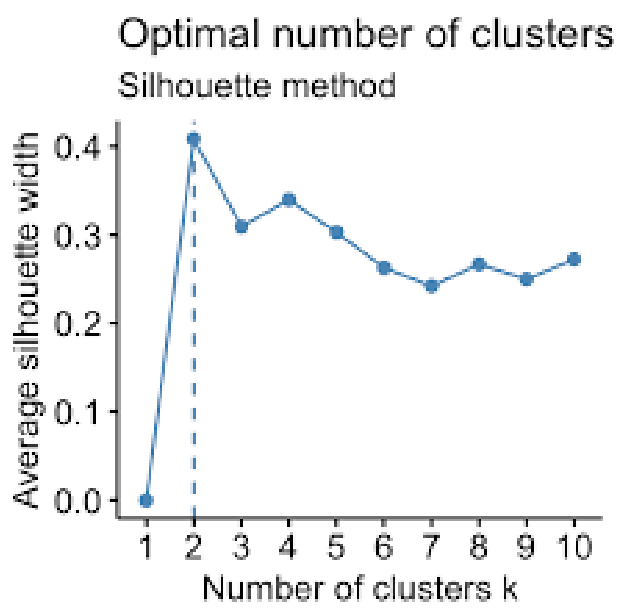
\includegraphics[scale=0.3]{images/silhouettemethod.png}
                    \caption{Plot the average silhouette coefficient according to an increasing number of clusters}
                    \label{fig:silhouette}
                \end{figure}
            \end{itemize}

    \section{Hierarchical clustering}
        This approach gives a lot of information about the structure of the data. The underline idea is that the groups often are hierarchical (as taxonomy). 
        There are two main greedy procedure to build hierarchical clustering: 
        \begin{enumerate}
            \item \textbf{Top-down approach}: starts with a single cluster and recursively splits the cluster in two groups according to a certain measure and then it repeats the procedure until we reach a maximum numbers of clusters or we reach clusters represented as single example.
            \item \textbf{Bottom-up approach}: starts with a number of clusters equal to the numbers of examples, and tries to merge the most similar clusters. Again, this procedure is recursive.
        \end{enumerate}

        This is something very common in computational biology, we end up with some kind of tree.
        The procedure for a bottom-up approach is pretty simple:
        \begin{enumerate}
            \item initialize:
            \begin{enumerate}
                \item final cluster number $k$ (the minimum final number of clusters)
                \item initial cluster number $\Tilde{k} = n$
                \item initial clusters $\mathcal{D}_i = \{ x_i \}, i \in 1, \dots, n$
            \end{enumerate}
            \item while $\Tilde{k} > k$:
            \begin{enumerate}
                \item find pairwise nearest clusters $\mathcal{D}_i, \mathcal{D}_j$ based on certain similarity measure
                \item merge $\mathcal{D}_i, \mathcal{D}_j$
                \item update $\Tilde{k} = \Tilde{k} - 1$
            \end{enumerate}
        \end{enumerate}

        The similarity measure is computed between clusters, there are several methods that we can use:
        \begin{itemize}
            \item nearest neighbours, computes the similarity between sets as the minimal distance between the elements in the two sets (sensible to outliers and expensive)
            \item furthest neighbors, computes the similarity between sets as the maximum distance between the elements in the two sets (sensible to outliers, expensive)
            \item average distance, computes the average distances between the elements in the two sets (expensive)
            \item distance between means of clusters (more efficient)
        \end{itemize}
        Each of this approaches has pros and cons, depending on the problem one way could be better than another. 
        We can also use some external and specific evaluation metric in order to find the clusters to merge (or to divide).
        This approach is \textbf{greedy} but not necessarily optimal. 